\chapter{Introduction}
\label{intro}
\par Almost 100 years ago on April 30th 1917 the Austrian mathematician Johann Radon described in "\"Uber die Bestimmung von Funktionen durch ihre Integralwerte l\"angs gewisser Mannigfaltigkeiten" the mathematical theory computed tomography is based on: He showed that the knowledge of a function \(f(x,y)\) in equivalent to the knowledge of all its line integrals. Thus the function can be reconstructed from an infinite set of its projections.\cite{Radon}
\par X-Ray is an imaging modality which produces projection images of a volume which show also the internals of the object. So in a perfect world by taking X-Ray images from all angles around an object orthogonal slices of the object can be reconstructed perfectly: In an idealized situation with high radiation dose, monochromatic X-Rays, infinite detector resolution, perfect detectors, no motion and no scatter CT images would be a perfect reflection of reality.\cite{CausesAndReductionTechniques}
\par In reality however these conditions are not met. Thus errors in the reconstruction occur resulting in image artefacts.
\par Usually especially for commercial CT scanners which are used in medical imaging the reduction of these artefacts is of special interest. But to better understand the causes of these artefacts as well as training of medical doctors to make reasonable diagnoses in the presence of these artefacts simulation is also of interest. In this clinical project we developed a simulator of a CT which produces CT images from segmented patient datasets in which the artefacts usually visible in medical imaging are also simulated in a realistic fashion. Especially the simulation of metal artefacts is of major importance as the resulting image artefacts are a major concern in medical imaging as these artefacts degrade image quality considerably.

\chapter{Causes of metal artefacts in CT}
\section{Examples of metal artefacts in CT}
\par To know why metal artefacts in CT should be simulated, we should first know what these metal artefacts are and how they look like.
\par The human body usually does not contain any metal objects. However many medical implants are composed of metal as well as many surgical tools. Thus metal can indeed be found quite often in patients who are scanned in CT scanners: Artificial hip bones, dental fillings, pacemakers, intramedullary rods, screws or in the case of inerventional CT surgical tools like needles, trocars etc. are found in many patients. If these patients are scanned in CT artefacts in the tomographic reconstruction are usually encountered, how severe these artefacts are depends mainly on their size and the material they are composed of.
\par These artefacts usually consist of dark stripes between metal objects with light, pin-striped lines covering the surrounding tissue going through the whole or large portions of the reconstruction as can be seen in figure \ref{BilateralHipReplacements}. Especially in cases in which the radiation is completely absorbed due to the thickness of the materials, very bright strips are found radially around the object with the complete image losing its diagnostic value. More examples can be found in appendix \ref{chapter:RealMetal}.
\begin{figure}[h!]
	\centering
	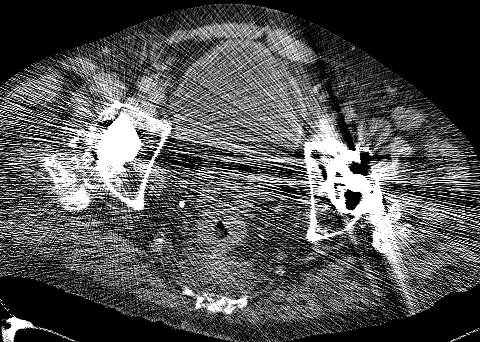
\includegraphics[width=0.5\linewidth]{images/12_FBP.png}
	\caption{Bilateral hip replacements (with streaks obscuring perirectal lymphadenopathy from rectal cancer)\cite{revisionrads}}
	\label{BilateralHipReplacements}
\end{figure}
\section{Fundamentals of X-Ray physics}
\par To understand the generation of CT metal artefacts we first need to understand how X-Ray generation and attenuation works in general.
\subsection{Generation of X-Ray radiation\cite{IIIP_3_1}}
\par To generate X-Ray radiation an X-Ray tube is used. It consists of a cathode and a rotating anode (usually made of tungsten) which is located within an evacuated tube housing. When electrons from the cathode hit the anode two physical effects take place which result in the emission of X-Ray radiation: Bremsstrahlung and characteristic X-Rays.
\par Bremsstrahlung results in a continuous spectrum of EM radiation which is produced by the abrupt deceleration of charged particles ("Bremsstrahlung" is German for "braking radiation"). This deceleration is caused by deflection of electrons in the Coulomb field of the nuclei of the anode material.
\par Characteristic rays are caused by the removal of inner shell electrons and subsequent filling of the holes with electrons from the outer shells. Shell energy differences determine the energies of the characteristic X-rays (this strongly depends on the anode material).
\par Both effects together result in the total emission spectrum of the X-Ray source. This spectrum depends on tube voltage and heating current and anode material and anode angle. This spectrum usually looks like as depicted in figure \ref{spectrum}.
\begin{figure}[h!]
	\centering
	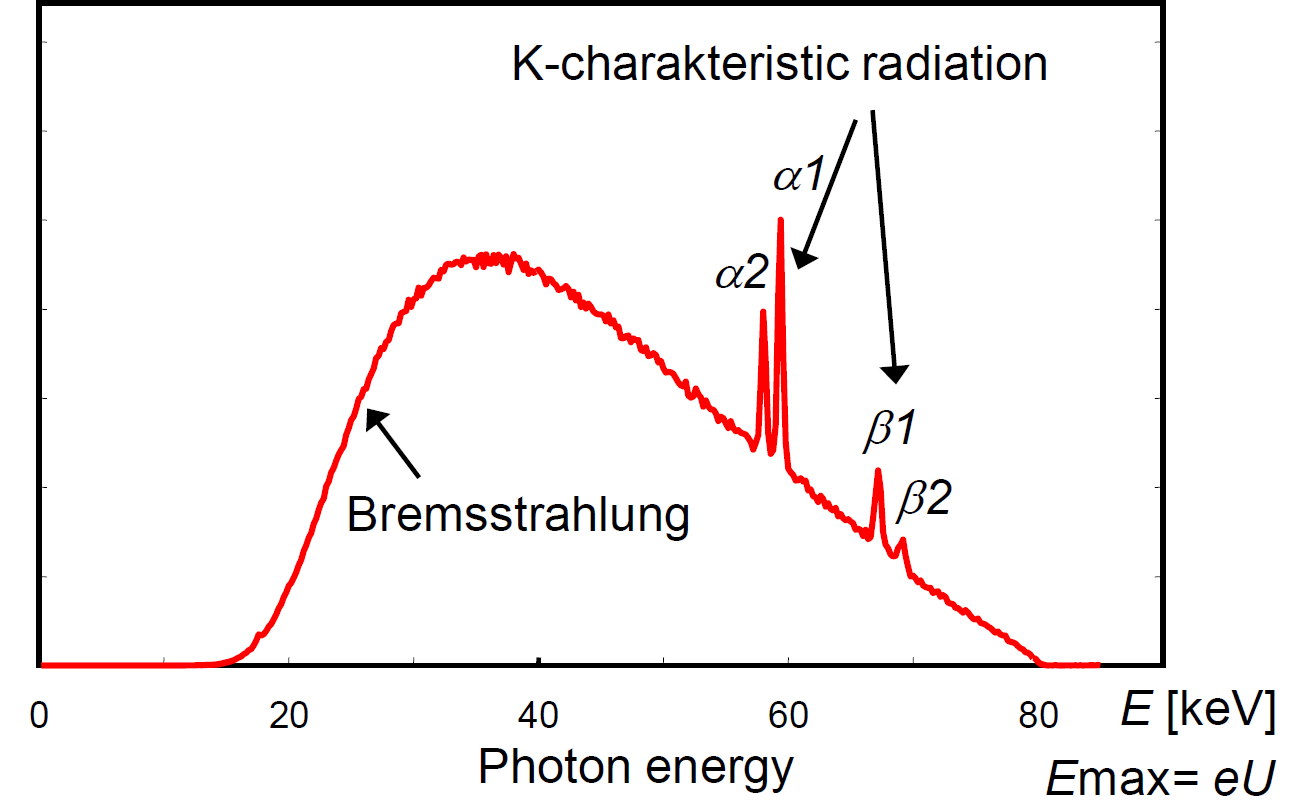
\includegraphics[width=0.9\linewidth]{images/spectrum.png}
	\caption{Total X-Ray spectrum of a tungsten anode at an acceleration voltage of \(U_a\) = 80kV\cite{IIIP_3_1}}
	\label{spectrum}
\end{figure}
\subsection{Lambert-Beer's Law\cite{buzug}}
\par Usually all physical mechanisms that lead to the attenuation of radiation intensity behind a homogeneous object are summed up in a single attenuation coefficient \(\mu\). In this simple model the total attenuation of a monochromatic X-Ray beam after passing a distance of \(\Delta\eta\) through an object can be calculated as \[I(\eta + \Delta\eta) = I(\eta) - \mu(\eta)I(\eta)\Delta\eta \] where \(I\) is the radiation intensity - which is proportional to the number of photons.
\par By reordering and taking the limit \(\Delta\eta \rightarrow 0\) this leads to the differential quotient\[\textrm{lim}_{\Delta\eta\rightarrow 0} \frac{I(\eta + \Delta\eta) - I(\eta)}{\Delta\eta} = \frac{\textrm{d}I}{\textrm{d}\eta} = -\mu(\eta)I(\eta)\]
\par If the medium is assumed to be homogeneous the medium can be described by a single attenuation constant \(\mu(\eta) = \mu\). By solving this ordinary linear and homogeneous, first-order differential equation with constant coefficients this gives the equation \[I(\eta) = I_{0}e^{-\mu\eta}\] know as Beer's law of attenuation.
\par The full derivation of the formula with all assumptions and mathematical intermediate steps can be found in \cite{buzug}.
\subsection{Beam hardening\cite{buzug}}
\par X-Ray is colloquially understood to have the property of effectively penetrating material. But from a physical point of view it can be seen that the radiation attenuation is not only dependent on path length but also wavelength dependent and also on the penetrated material.
\par Thus Lambert-Beer's Law is indeed a simplification. The energy dependence of the attenuation coefficient along the path \(s\) also has to be taken into consideration \(\mu = \mu(\eta,E)\). This leads to \[I(s) = \int_0^{E_{\textrm{max}}}I_0(E)e^{-\int_0^{s}\mu(\eta,E)\textrm{d}\eta}\textrm{d}E\] where \(I_0(E)\) is the X-Ray spectrum.
\par Reconstruction does not take this non-linear relationship due to the fact that different bands of the frequency spectrum are differently attenuated between the attenuation values, \(\mu\), and the measured values of the projection into account thus impairing the reconstruction.
\par Soft X-ray beams are more strongly absorbed than high-energy, \emph{hard} X-Ray beams. The individual detector elements in practice only measure the integral intensity over all wavelengths, i.e., they cannot differentiate distinct energies. If a non monochromatic X-Ray beam passes through an object different bands of its spectrum are differently attenuated. Without taking this into account in the reconstruction this leads to so called beam hardening artefacts.
\par The beam hardening effect is especially prominent for metals that are introduced into the human body as their atomic number Z is relatively high with absorption given by \[\alpha \propto Z^4\lambda^3\] (Due to this relationship for example lead (Pb, Z = 82) shields X-ray radiation about 1583 times better than aluminium (Al, Z = 13))
\par Thus behind a thick metal object the system detects an \emph{infinitely high} attenuation coefficient. Filtered backprojection does not cope with the inconsistencies in the attenuation values. In the backprojection lines through the object are encountered with extremely high numerical values, which spread across the entire image and are not compensated for by any other projection direction creating star like streaks emanating from the metal object going through the whole or large portions of the reconstruction.\cite{buzug}
\section{Fundamentals of CT reconstruction}
\subsection{Sinograms}
\par As described in section \ref{intro} the knowledge of all line integrals of \emph{projections} of a function \(f(x,y)\) is equivalent to the knowledge of the function itself. With X-Ray being able to create projections of objects opaque to the human eye with this theorem we can create axial slices (or tomographies from \(\tau\acute{o}\mu o\varsigma\) \emph{tomos}, "slice, section" and \(\gamma\rho\acute{\alpha}\varphi\omega\) \emph{gr\'aph\=o}, "to write"\cite{wiktionaryTomography}\cite{wiktionaryTomo}\cite{wiktionaryGraphy}) when we take X-Rays from all angles around the object.
\par An image of all the projections from a line detector of a single slice of an object is called \emph{sinogram} or mathematically Radon transform: In one axis of the image the angle is gradually increased and along the perpendicular line the projection values from the line detector is plotted.
\par In figure \ref{shepplogan} the famous Shepp-Logan phantom can be seen created by Larry Shepp and Benjamin F. Logan which serves as a crude model of a human head to develop and test image reconstruction algorithms on. Figure \ref{shepplogansino} is the sinogram of this phantom.\cite{shepploganphantom}
\begin{figure}[h!]
	\centering
	\begin{subfigure}[b]{0.28\textwidth}
		\centering
		\includegraphics[height=4cm]{images/shepp_logan.png}
		\caption{The famous Shepp Logan phantom (own work, based on \cite{shepploganphantom})}
		\label{shepplogan}
	\end{subfigure}%
	~
	\begin{subfigure}[b]{0.68\textwidth}
		\centering
		\includegraphics[height=4cm]{images/shepp_logan_sino.png}
		\caption{Sinogram of the Shepp Logan phantom (own work, based on \cite{shepploganphantom}): In Y direction the projection angle around the object in increased, in X direction the values of the detector are plotted.}
		\label{shepplogansino}
	\end{subfigure}%	
\end{figure}
\subsection{Simple Backprojection}
\par To transform such a sinogram from \(p_\gamma(\xi)\) back into the image space \(f(x,y)\) the basic idea is to \emph{backproject} the values of the detector line along the angle these were acquired from into the image. In the case of \emph{simple backprojection} the would be to \emph{smear back} the values in the direction from which the radiation came. However, although intuitively thsi simple backprojection seems to reverse the process of projection, this procedure does not result in the desired outcome: Due to the fact that the projection \(p_\gamma(\xi)\) is a non-negative
function, the simple backprojection smears back non-negative values over the entire image, even in areas that were originally (close to) zero. The backprojections from other directions cannot correct these incorrect pixel entries, because the entire set of projections in the sinogram is a set of non-negative functions. Simple backprojection is visualized in \ref{zeng1} and \ref{zeng2} showing that it would result in an overall unacceptable blurring of the image.\cite{buzug}
\begin{figure}[h!]
	\centering
	\begin{subfigure}[b]{0.5\textwidth}
		\centering
		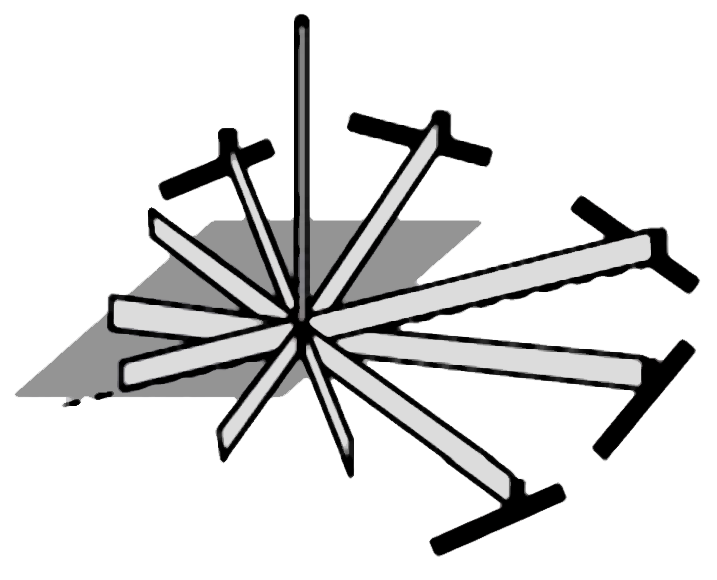
\includegraphics[height=3cm]{images/zeng1_Shopped.png}
		\caption{The simple backprojection of a single point...\cite{zeng}}
		\label{zeng1}
	\end{subfigure}%
	~
	\begin{subfigure}[b]{0.5\textwidth}
		\centering
		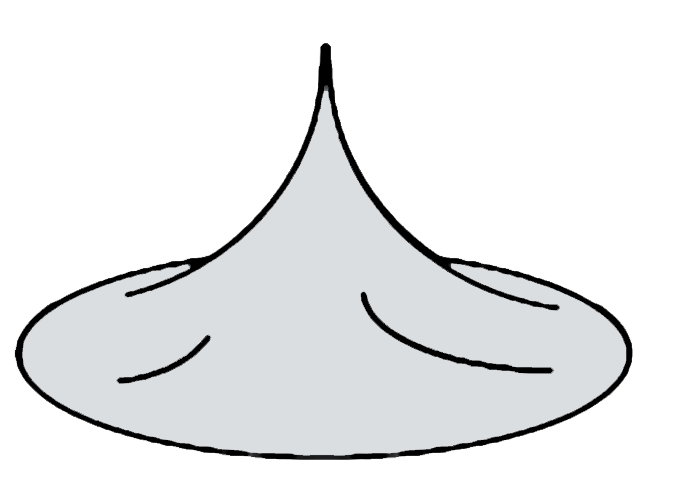
\includegraphics[height=3cm]{images/zeng2_Shopped.png}
		\caption{...would result in the pointspread function of a single point.\cite{zeng}}
		\label{zeng2}
	\end{subfigure}%
\end{figure}
\subsection{Filtered Backprojection}
\par To correct for this unacceptable blurring so called \emph{filtered backprojection} is employed. Today all modern CT systems implement filtered backprojection (and other more advanced reconstruction algorithms). Essentially before backprojecting a high-pass filter is applied. Graphically this can be seen as adding \emph{"negative wings"} to the projections as can be seen in \ref{zeng3} and \ref{zeng4}. For a mathematical explanation of filtered backprojection and why this is in fact a suitable inversion of the Radon Transform refer to \cite{buzug}.
\begin{figure}[h!]
	\centering
	\begin{subfigure}[b]{0.5\textwidth}
		\centering
		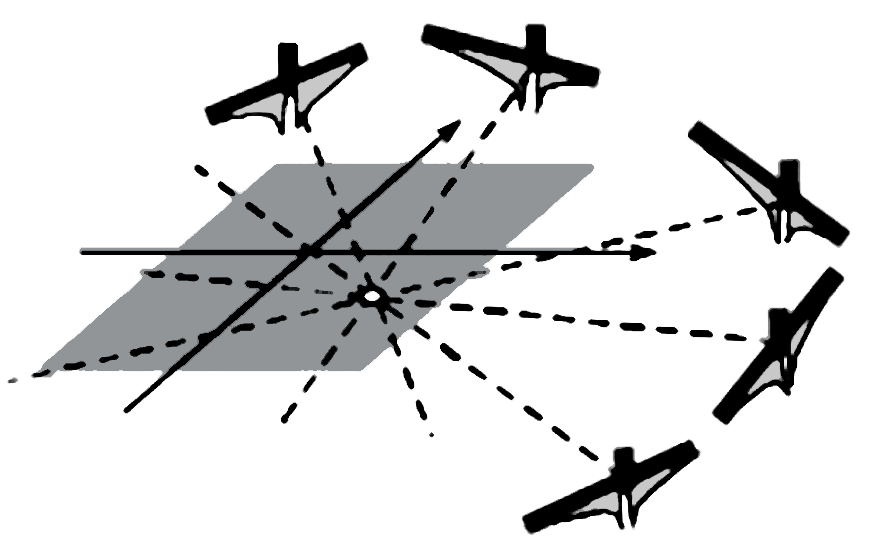
\includegraphics[height=3cm]{images/zeng3_Shopped.png}
		\caption{Applying a high-pass filter before projection ...\cite{zeng}}
		\label{zeng3}
	\end{subfigure}%
	~
	\begin{subfigure}[b]{0.5\textwidth}
		\centering
		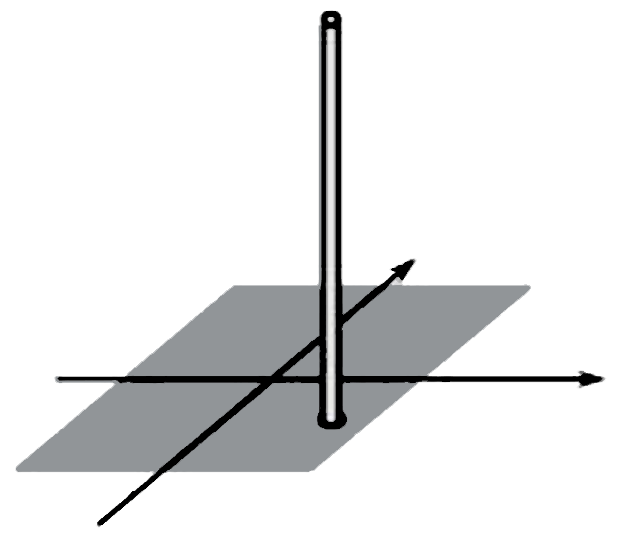
\includegraphics[height=3cm]{images/zeng4_Shopped.png}
		\caption{...results in a crisp reconstruction of the tomography.\cite{zeng}}
		\label{zeng4}
	\end{subfigure}%
\end{figure}
\par Generally the inversion of the Radon transform is an ill-posed problem because the solution is not a continuous function. There are however other techniques for reconstruction, like algebraic and statistical methods and iterative methods.\cite{SchlechtGestellteProbleme}\cite{buzug}
\par But filtered backprojection is still used in practice as it is computationally fast. Also for our purposes it is the backprojection method of choice as beam hardening and metal artefacts are more prominent than for example in iterative reconstruction.\cite{buzug}

\chapter{Simulation of CT}
\par In general the simulation of computed tomography consists of two parts: Forward projection and backprojection.
\par For this clinical project a CT simulator was programmed from ground up in the C programming language without any major libraries like OpenCV, OpenGL or OpenMP. Only standard libraries like \verb!Math.h!, \verb!stdio.h!, \verb!stdlib.h! and the like were included as well as \verb!windows.h! for performance measurements and basic multi threading.
\par The reason for the decision on C was that originally it was intended to port the code to CUDA-C for calculation on the graphics card to boost performance by multiple orders of magnitude. However due to the lack of time, experience and access to a PC with an NVidia graphics card this port was not completed. Generally the problem seems to be well suited for computation on the graphics card as every forward projection can be calculated in parallel, as well as the filtered backprojection which can also be sped up on the graphics card by a factor of over 200.\cite{CUDABackprojection}.
\par The source code for this simulator is available in a git repository hosted at GitHub. It can be found in \url{https://github.com/Axelius/CTSim.git}
\section{Forward Projection}
\par The forward projection is in essence a forward Radon Transform with some special conditional statements to simulate effects that exist in physical reality but not in the mathematical model. The simulation especially focuses on the effects of beam hardening, so it simulates a virtual X-Ray tube and has lookup tables for attenuation values of different materials at different tube voltages.
\par For this simulator basic parallel beam CT was chosen, although today fan beam or cone beam geometry is state of the art. But the artefacts in fan beam geometry should be the same as in parallel beam geometry as fan beam can be converted to parallel beam by simple reordering of the X-Ray beams.\cite{IIIP_3_4} In cone beam geometry no central slice theorem exists anyway, so reconstruction is \emph{not mathematically correct anyway} so the simulation of this was not considered\cite{IIIP_3_5}.
\par To sum it up the forward projection can be formulated as the formula\[\sum_{p\in P}\sum_{en\in E}\sum_{d \in D}\sum_{l \in L}I_{0}\cdot \textrm{e}^{-\sum_{\eta \in M}\mu(\eta,x,y,en)}\] where \(p\in P\) is the projection angle, \(en\in E\) the energy level, \(d \in D\) the detector element, \(l \in L\) the length of the ray after leaving the X-Ray source and \(\eta \in M\) the material. \(x\) and \(y\) is the position of the currently examined pixel that is calculated from the projection angle, detector element and ray length as \(x = l\cdot sin(p) + d\cdot cos(p)\) and \(y = -l\cdot cos(p) + d\cdot sin(p)\). The general idea and the proof that CT can be simulated in this was is from \cite{deMan}. However they did their sum slightly different and in a different order. Still, this thesis was very helpful as a basis for how to tackle simulation of CT.
\subsection{Overview over the forward projection}
\begin{figure}[h!]
	\centering
	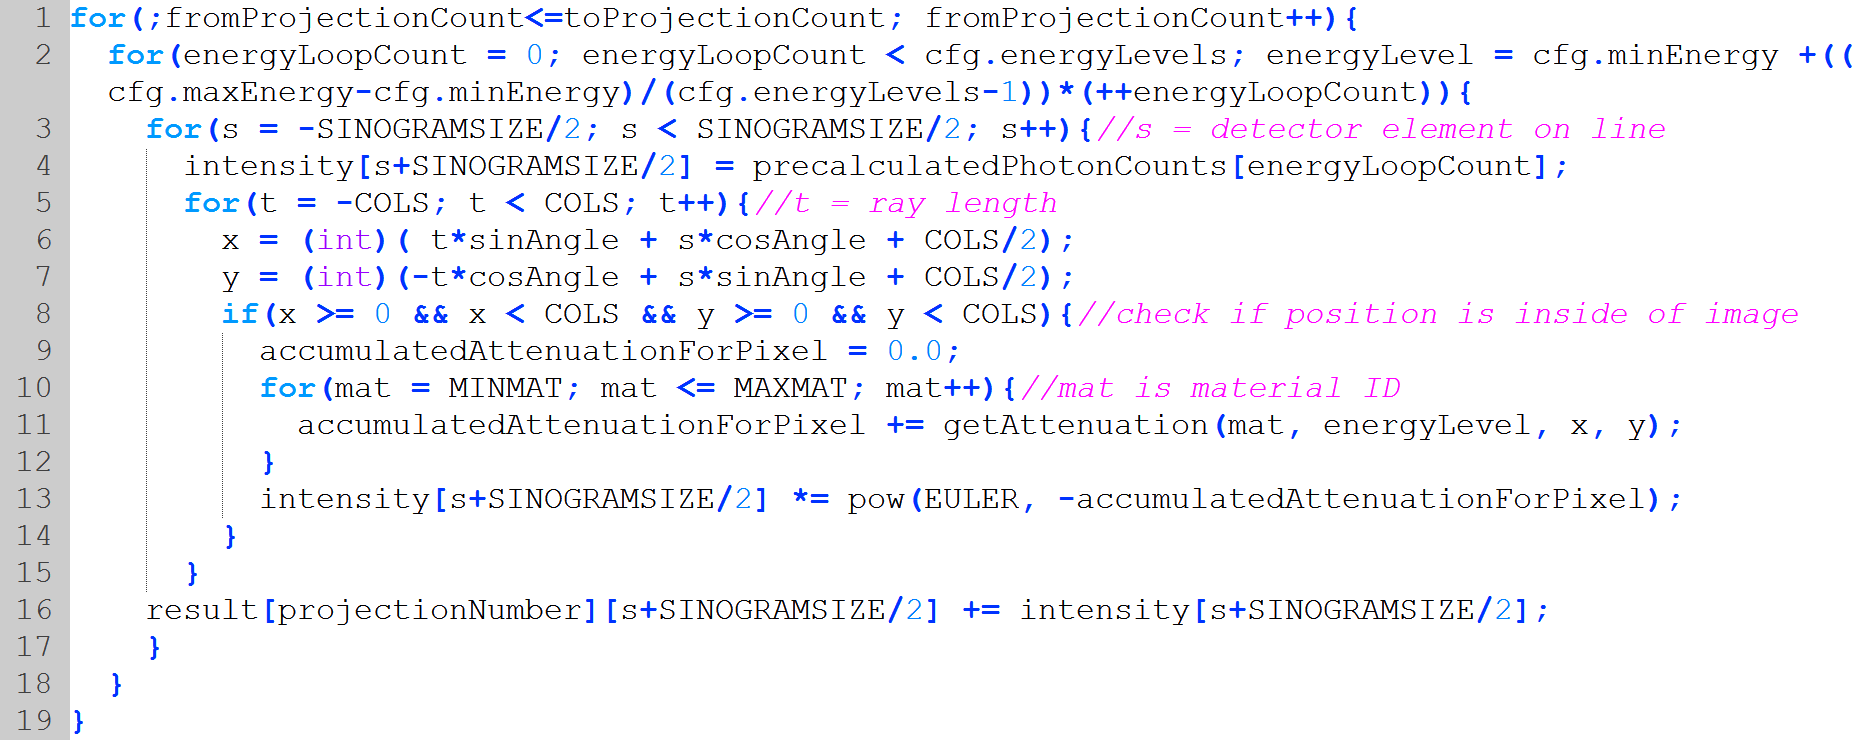
\includegraphics[width=\linewidth]{images/MainLoop.png}
	\caption{Translation of the formula to source code}
	\label{MainLoop}
\end{figure}
\par Figure \ref{MainLoop} shows a pseudo code snipped which was slightly modified from the simulation C code. It shows how the above mentioned formula translates to C style pseudo code.
\par As mentioned above the forward projection is essentially a Radon Transform with some additions: Polychromaticity is modelled by summing a number of monochromatic simulations which makes it necessary to have a virtual model of the X-Ray tube spectrum (in this case simple lookup tables for different tube voltages). Also as X-Ray photons are differently attenuated at different energy levels for different materials another loop was included to loop over that materials. For the attenuation coefficients lookup tables for different materials were created from \cite{AttenuationTable} between whose values we interpolate linearly.
\par The forward projection returns a sinogram of the specified object. This sinogram can then be passed to the backprojection for reconstruction.
\par The source code for the forward projection is located in \verb!simulator.c!. The method \verb!int project(int projectionNumber, double angle)! calculates one complete projection for the specified angle and saves its result to \verb!result[projectionNumber]!. This method is called for every projection until the complete 180\textdegree of the projection is completed. A specified number of threads calls this function, but no race conditions have to be expected as every thread has its own range of projection angles and writes only to his own range of the array \verb!result!. As every thread has approximately the same number of projections and every projection takes about the same time no dynamic job distribution was needed and in the beginning the projections are statically distributed on the threads.
\subsection{Implementation of line integrals}
\par The calculation of line integrals is a straightforward discretization of the Radon transform: The integral is approximated by a sum of the attenuation values.
\par As mentioned above we assume parallel beam geometry. Although in the 2D case fan beam geometry is state of the art (parallel beam was only common in the first generation of CTs) mathematically this is equivalent: Fan beam geometry can be transformed to parallel beam geometry by reordering of the beams.\cite{IIIP_3_4}
\par So in parallel beam geometry every detector element has a perpendicular ray passing through the object. At the beginning this ray has the intensity \(I_{0}\) which is the the number of X-Ray photons described by the tube spectrum. This spectrum is dependent on the tube voltage, so we have implemented different spectra for common tube voltages of 80keV to 140keV from which the closest to the selected voltage is selected.
\par This ray passes through the object. After every pixel the intensity is reduced according to the attenuation value of this pixel. This pixel's attenuation is a sum of all the single attenuation values of the materials that are present at this pixel.
\subsection{Implementation of beam hardening}
\par As mentioned above in the mathematical model of Radon transform beam hardening does not exist but in reality it does as the detector basically measures an attenuation of \emph{infinity} (or at least very high numerical values). To simulate this behaviour the attenuation is simply capped at a certain value to simulate the fact that the ray has lost all its energy.
\par Especially for beam hardening the X-Ray tube model was created as the shift of the spectrum after passing through an object is the main reason for beam hardening which could not be modelled realistically with equally distributed intensity over all energies.  
\section{Backprojection}
\par Backprojection is not really a simulation task as this has to be done in real CTs too. Thus not much time was spent on it and a nice implementation from \cite{CUDABackprojection} was adapted which implements a filtered backprojection in C. Moreover \cite{CUDABackprojection} describes how this algorithm can be ported to CUDA-C for execution of the graphics card which experimentally resulted in a speedup of over 200. Computation speed comparison is visualized in figure \ref{ArnesenSpeedup}.
\begin{figure}[h!]
	\centering
	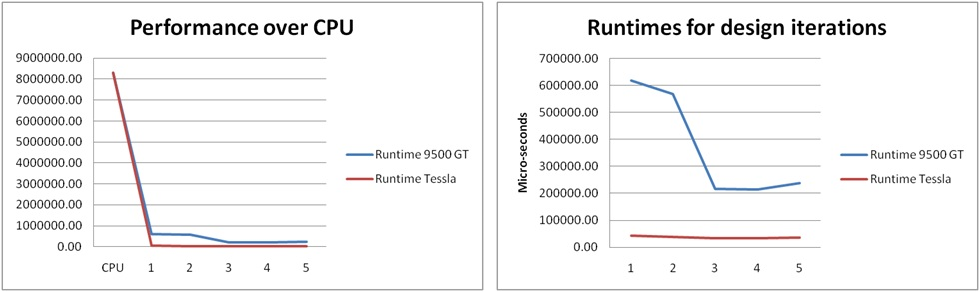
\includegraphics[width=\linewidth]{images/ArnesenSpeedupCombined.png}
	\caption{Computation time of the reconstruction algorithm using calculation on the CPU and on the graphics card in 5 algorithm iterations\cite{CUDABackprojection}}
	\label{ArnesenSpeedup}
\end{figure}
\section{Parts of the simulator}
\par In this section we will have a closer look at the parts of the simulator other than forward projection and backprojection.
\subsection{Segmented CT slice}
\par The simulation of course needs information about the object to be "scanned" and reconstructed. As we use 2D parallel beam geometry a segmented 2D slice of the object to be simulated is sufficient. If one desires to create a whole volume several runs on successive slices can be performed using a batch file etc.
\par The simulation accepts folders as input of the segmentation with separate image files for each material. They have to be in \verb!pgm! format and named \verb!air.pgm!, \verb!bone.pgm!, \verb!iron.pgm!, \verb!muscle.pgm!, \verb!tissue.pgm! and \verb!water.pgm! respectively as their name is hardcoded. In these single images white corresponds to the existence of this material on the respective position, black corresponds to the lack of this material on this position. Grey values correspond to intermediate values the simulation simply multiplies the grey value with the corresponding attenuation coefficient.
\par The segmentation that was mainly used for development is based on an abdominal slice of the Visible Korean Human Project\cite{visibleKorean} in which arbitrarily a single metal object was placed close to the center. All the slices can be seen in figures \ref{korean1}, \ref{korean2}, \ref{korean3}, \ref{korean4}, \ref{korean5} and \ref{korean6}.
\begin{figure}[h!]
	\centering
	\begin{subfigure}[h]{0.3\textwidth}
		\centering
		
\includegraphics[height=4cm]{images/KoreanAir.png}
		\caption{The air surrounding the dataset}
		\label{korean1}
	\end{subfigure}%
	~
	\begin{subfigure}[h]{0.3\textwidth}
		\centering
		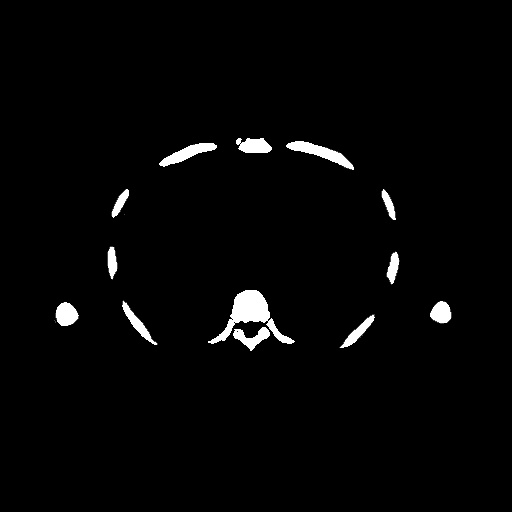
\includegraphics[height=4cm]{images/KoreanBone.png}
		\caption{The bones of the dataset\linebreak}
		\label{korean2}
	\end{subfigure}%
	~
	\begin{subfigure}[h]{0.3\textwidth}
		\centering
		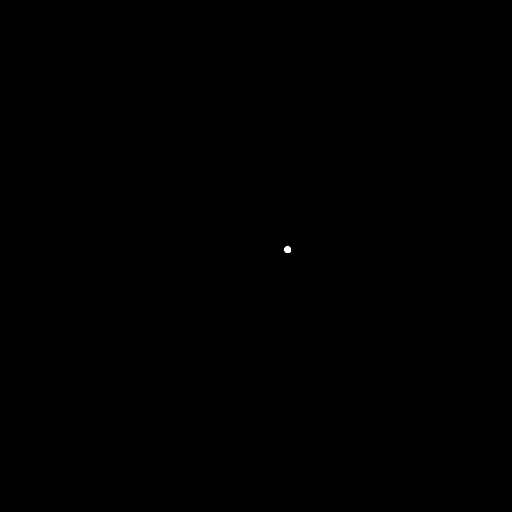
\includegraphics[height=4cm]{images/KoreanIron.png}
		\caption{The arbitrarily set iron object inside the dataset}
		\label{korean3}
	\end{subfigure}%
	
	\begin{subfigure}[h]{0.3\textwidth}
		\centering
		
\includegraphics[height=4cm]{images/KoreanMuscle.png}
		\caption{The muscular structures of the dataset\\}
		\label{korean4}
	\end{subfigure}%
	~
	\begin{subfigure}[h]{0.3\textwidth}
		\centering
		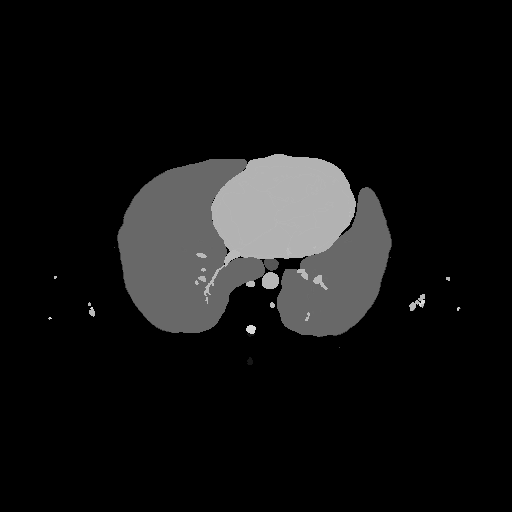
\includegraphics[height=4cm]{images/KoreanTissue.png}
		\caption{Tissue material of the dataset\\}
		\label{korean5}
	\end{subfigure}%
	~
	\begin{subfigure}[h]{0.3\textwidth}
		\centering
		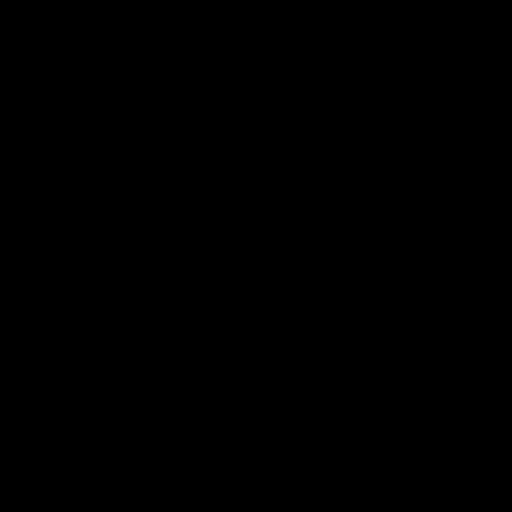
\includegraphics[height=4cm]{images/KoreanWater.png}
		\caption{Water can also be placed in the simulation but in this case we didn't.}
		\label{korean6}
	\end{subfigure}%
\end{figure}
\subsection{Simulation of an X-Ray tube}
\par As mentioned before for a realistic simulation of beam hardening a virtual model of the X-Ray tube spectrum is needed.\cite{XRayTubeSpectrum}
\par For this we simulation we use lookup tables based on \cite{XRayTubeSpectrum}. They provide relative photon counts of an X-Ray tube at different tube voltages which is also visualized in \ref{f5}. From this we created separated lookup tables for each tube voltage. For the use in our simulation we sampled the spectrum at intervals of 5keV resulting in \ref{SampledTubeSpectrum}. The relative X-Ray photon count is then used as the intensity \(I_{0}\) of the ray leaving the X-Ray tube. After passing through each pixel of the simulation area this intensity is reduced as suggested by Lambert-Beer's Law.
\begin{figure}[h!]
	\centering
	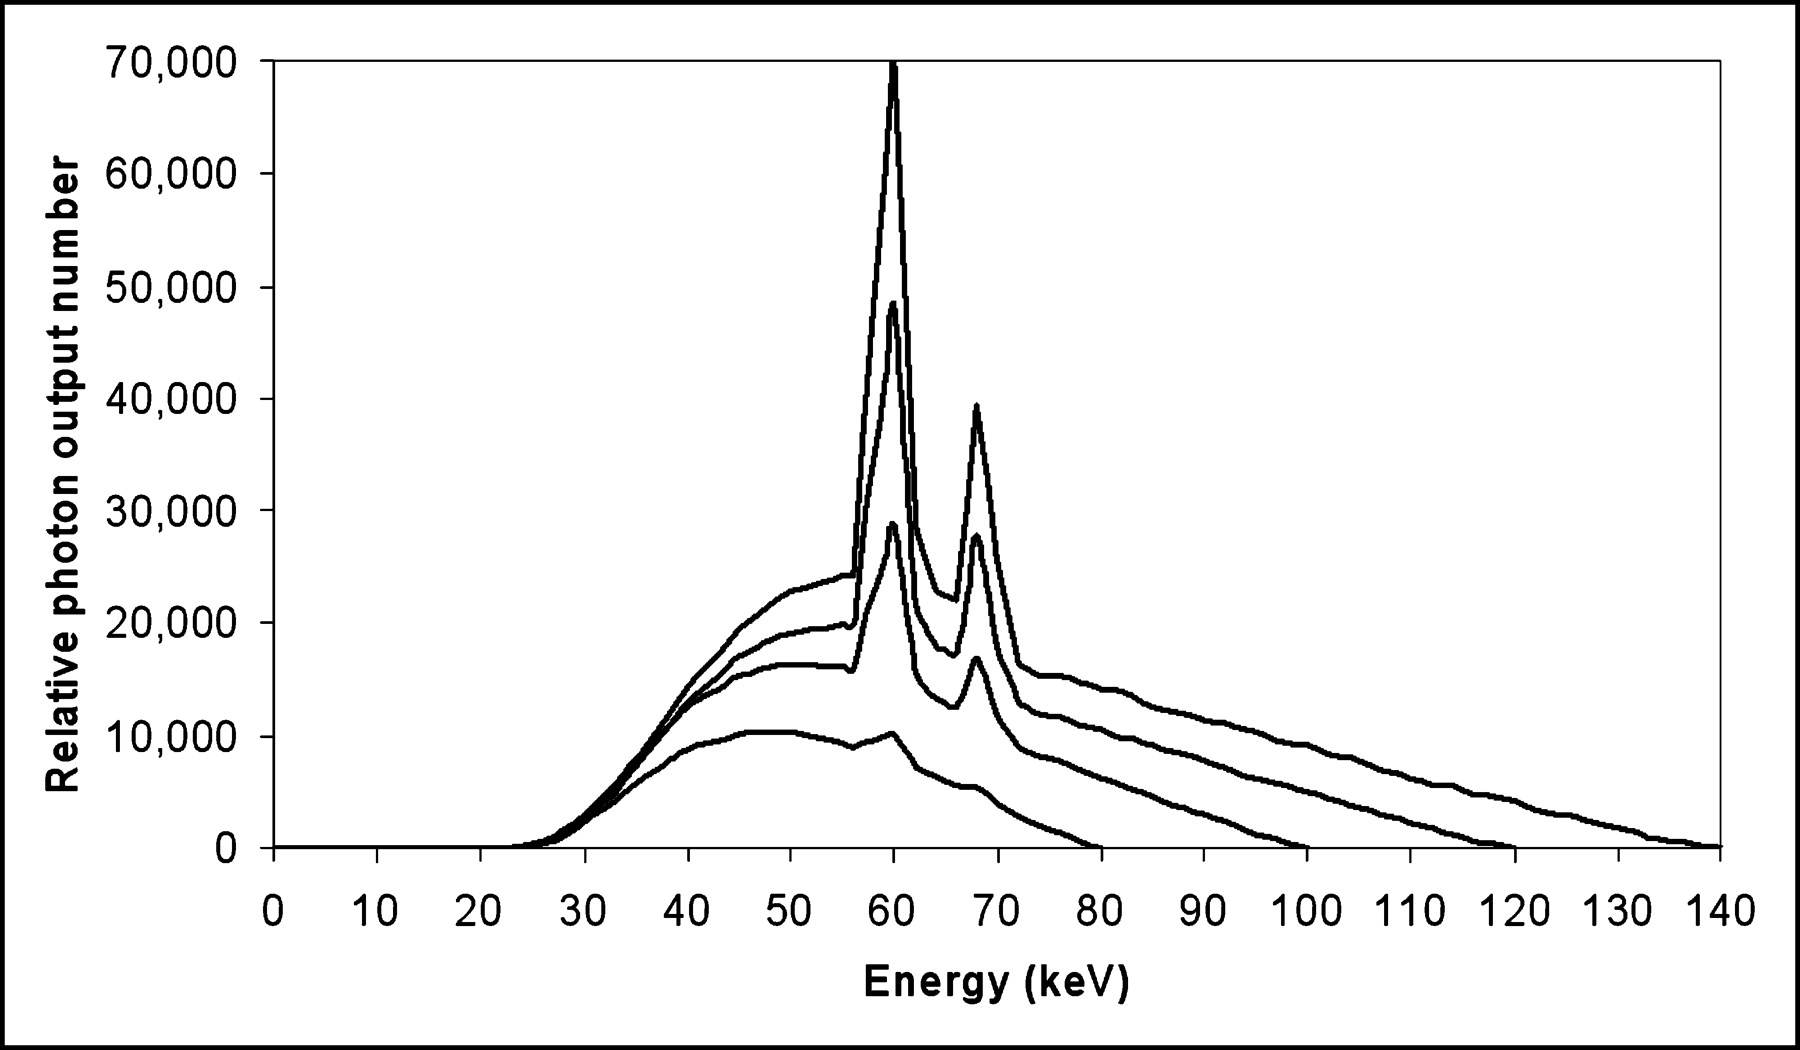
\includegraphics[width=0.6\linewidth]{images/F5large.jpg}
	\caption{Spectrum of an X-Ray tube at different tube voltages\cite{XRayTubeSpectrum}}
	\label{f5}
\end{figure}
\begin{figure}[h!]
	\centering
	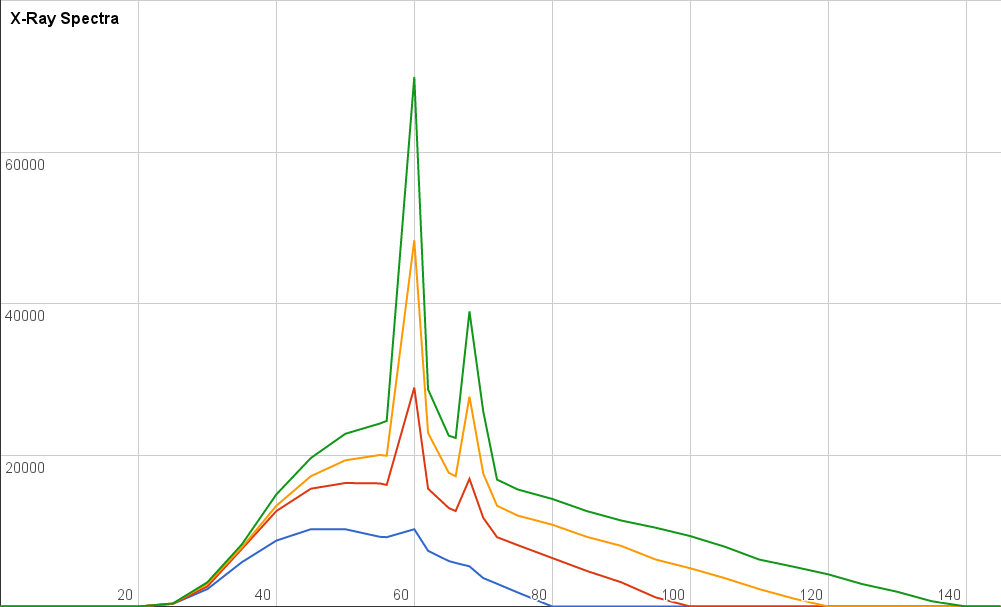
\includegraphics[width=0.5\linewidth]{images/tubeSpectrum.png}
	\caption{Sampled X-Ray spectrum at equal distances of 5keV.}
	\label{SampledTubeSpectrum}
\end{figure}
\subsection{Lookup tables for attenuation values}
\par Different materials have different attenuation values. As mentioned before the attenuation value is dependent on the atomic mass \(Z\) but also on the density of the material. For our simulation we relied on measurements of \cite{AttenuationTable} who provide attenuation values for different elements but also compounds, mixtures and various human tissues at different photon energies. A visualization of such a table can be seen in figure \ref{muscleAtt}.
\begin{figure}[h!]
	\centering
	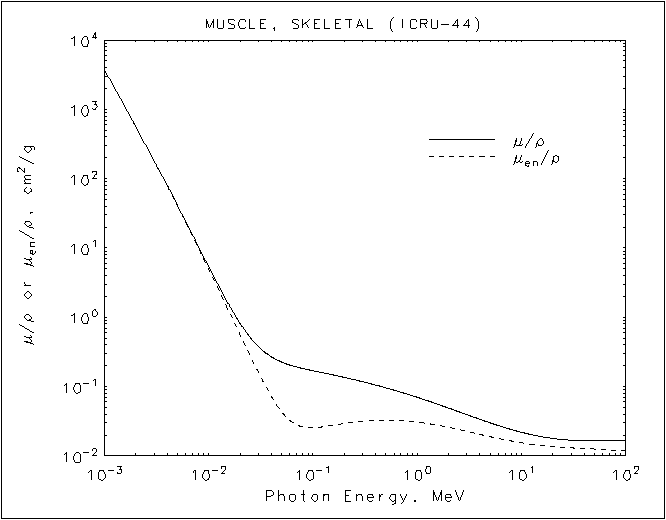
\includegraphics[width=0.5\linewidth]{images/muscle.png}
	\caption{X-Ray Mass Attenuation Coefficients of skeletal muscle\cite{AttenuationTable}}
	\label{muscleAtt}
\end{figure}
\par At each position of the simulation the intensity \(I_{0}\) of the photons of a certain energy level is reduced according to the attenuation which is linearly interpolated from these lookup tables. If the grey value in the segmentation is not pure white the corresponding value is multiplied by the ratio between the grey value and pure white.
\subsection{Configuration file}
\par The simulation can be configured using a simple configuration file like can be seen in listing \ref{configfile}.
\lstset{ %
  basicstyle=\footnotesize,
}
\begin{lstlisting}[caption={Sample configuration file},label=configfile,captionpos=b]
pathToSlice=slices/Segmentation1
pathToOutputReconstruction=outData.pgm
pathToOutputSinogram=simulatedSinogram.pgm
pathToXRaySpectra=Data/XRaySpectra
minEnergy=20
maxEnergy=140
energyLevels=16
numberOfProjectionAngles=64
numberOfThreads=4
tubeEnergy=140
detectorThreshold=100
attenuationMultiplicator=40
\end{lstlisting}
\par We will look at each entry separately:
\begin{itemize}
	\item\emph{pathToSlice}: Path to the folder in which the segmentation of the slice to be rendered is located. This folder should contain several \verb!.pgm! files named \verb!air.pgm!, \verb!bone.pgm!, \verb!iron.pgm!, \verb!muscle.pgm!, \verb!tissue.pgm! and \verb!water.pgm! respectively.
	\item\emph{pathToOutputReconstruction}: Path to a \verb!.pgm! file to which the reconstruction is to be saved.
	\item\emph{pathToOutputSinogram}: Path to a \verb!.pgm! file where the intermediate simulated sinogram is to be saved. Even if you are not interested in the sinogram only in the reconstruction a path has to be set, as the reconstruction only accepts an image and can't directly read the sinogram from RAM.
	\item\emph{pathToXRaySpectra}: Path to where lookup tables for the X-Ray spectra are located. These should be named \verb!XRaySpectrum80keV.txt!, \verb!XRaySpectrum100keV.txt!, \verb!XRaySpectrum120keV.txt! and \verb!XRaySpectrum140keV.txt! as their name is hardcoded. The files themselves are simple textfiles with each line stating a certain energy and the corresponding relative photon count.
	\item\emph{minEnergy}: Minimum energy in keV of the photons leaving the X-Ray tube. As Polychromaticity is simulated as a number of monochromatic simulation runs this is the lowest energy that is simulated. No photons are generated with an energy lower that this value.
	\item\emph{maxEnergy}: Maximum energy in keV of the photons leaving the X-Ray tube. As polychromaticity is simulated as a number of monochromatic simulation runs this is the highest energy that is simulated. No photons are generated with an energy higher that this value.
	\item\emph{energyLevels}: Number of monochromatic simulation runs to simulate polychromaticity. Higher values result in a better approximation of polychromaticity. Computation time is however direct proportional to the number of energy levels.
	\item\emph{numberOfProjectionAngles}: Number of projections. With low values severe undersampling artefacts are encountered, high values result in smooth reconstructions. But beware that computation time is direct proportional to the number of projections.
	\item\emph{numberOfThreads}: Number of threads for the forward projection. This should be the same number as cores in the computer that runs this program for maximum speedup. Computation time is almost indirect proportional to the number of threads if the number of threads is equal to the number of cores, higher values usually result in no speedup or even an increase in computation time. Note that the backprojection always only uses one thread (but as this part of the simulation only takes a few seconds this time should be negligible).
	\item\emph{tubeEnergy}: Tube energy of the simulated X-Ray tube. For this only values of 80kev, 100keV, 120keV and 140keV are accepted, as only for these tube energies lookup tables exist. However these are reasonable values for medical X-Ray. If other values are set the closest match to the existing lookup tables is selected.
	\item\emph{detectorThreshold}: Threshold of photon count below which the beam is assumed to have completely starved. No further simulation of the ray is carried out below this value. Higher values can result in more severe metal artefacts, but too high values result in completely images (as the X-Ray beam coming from the tube may already be below this threshold).
	\item\emph{attenuationMultiplicator}: Multiplication factor of the attenuation coefficient. While not physically correct by tweaking this value sometimes more severe metal artefacts can be created. But as with the value before too high values might result in blank images as almost every ray is completely absorbed.
\end{itemize}
\par The simulation accepts the configuration file as the first parameter of the call to the executable. Note that reading theses configuration files is not too stably implemented and it it generally a good idea not to change the structure of these files but only set different values. Especially the value of each field should follow directly after the "\(=\)" sign without a whitespace in between.
\section{Miscellaneous parts of the simulator}
\par There are also some parts not directly related to the simulation of CT metal artefacts. But as the paradigm of this program was not to rely on any external libraries some more code had to be implemented. 
\subsection{Logger}
\par We implemented a simple logger to produce structured terminal output similar to libraries like log4j\cite{ApacheLog4j}. With such a logging framework you can \emph{plaster} your source code with logging statements, but select in which \emph{loglevel} you are interested in and only produce output of this loglevel (or higher). By specifying the current loglevel as a macro no messages with a lower loglevel will be produced.
\par By heavily relying on macros messages on a lower loglevel hardly influence computation time as the method immediately returns.
\par Messages can be filtered by loglevel according to their importance. The general order of these levels is: \[\verb!ALL > TRACE > DEBUG > INFO > WARN > ERR > FATAL > OFF!\] As a guideline these levels should be used as follows (inspired by the guidelines of log4j\cite{ApacheLog4jLevels}):
\begin{itemize}
	\item\emph{ALL}: No messages are filtered displaying all.
	\item\emph{TRACE}: Elaborate debugging and comments
	\item\emph{DEBUG}: General debugging and detailed information on the flow through the system
	\item\emph{INFO}: General information like \verb!"program started"!, \verb!"program closed"!,\\ \verb!"Computation took that many seconds"! etc.
	\item\emph{WARN}: Occurrence of runtime situations that are undesirable or unexpected, but not necessarily "wrong"
	\item\emph{ERR}: Error, but execution continues
	\item\emph{FATAL}: Critical errors that cause premature termination
	\item\emph{OFF}: No messages will be printed, logging deactivated
\end{itemize}
\par The implemented logger can output its messages to the console or to a file. To file can be especially useful on higher loglevels as the output to the console of thousands of messages can really slow down the program execution.
\par Moreover the logger can produce verbose or non verbose messages. In non verbose mode only the loglevel and message are printed, in verbose mode loglevel, source code file, function, line and message. So the call to \[\verb!logIt(INFO, "Starting simulation...")!\] results in non verbose mode in \[\verb![LogIt-INFO ] Starting simulation...!\] and in verbose mode in \[\verb![[LogIt-INFO ][..\src\Run.c].main.31] Starting simulation...!\] when it was called from the method \verb!main! in source code file \verb!Run.c! on line 31.
\par The logger is completely independent in the source code files \verb!Logger.h! and \verb!Logger.c!, relies only on \verb!stdio.h!, \verb!stdarg.h! and \verb!String.h! and can be put in any C project by including \verb!Logger.h!.
\subsection{Image reading and writing}
\par As mentioned before we did not want to rely on any external libraries other than the standard libraries. So for image import and export we chose one of the easiest image file formats available which is the portable graymap format \verb!.pgm! which belongs to Portable Anymap or Netpbm format.
\par In Portable GrayMap with the magic number \verb!P2! a simple and short header is followed by the greyvalues in ASCII in the range \(0-255\).
\par An example from the Netpbm man page on PGM can be seen in listing \ref{feep1} with its graphical representation in figure \ref{feep2}
\begin{lstlisting}[caption={PGM example from the Netpbm man page on PGM\cite{pgmNetPBM}},label=feep1,captionpos=b]
P2
# feep.pgm
24 7
15
0  0  0  0  0  0  0  0  0  0  0  0  0  0  0  0  0  0  0  0  0  0  0  0
0  3  3  3  3  0  0  7  7  7  7  0  0 11 11 11 11  0  0 15 15 15 15  0
0  3  0  0  0  0  0  7  0  0  0  0  0 11  0  0  0  0  0 15  0  0 15  0
0  3  3  3  0  0  0  7  7  7  0  0  0 11 11 11  0  0  0 15 15 15 15  0
0  3  0  0  0  0  0  7  0  0  0  0  0 11  0  0  0  0  0 15  0  0  0  0
0  3  0  0  0  0  0  7  7  7  7  0  0 11 11 11 11  0  0 15  0  0  0  0
0  0  0  0  0  0  0  0  0  0  0  0  0  0  0  0  0  0  0  0  0  0  0  0
\end{lstlisting}
\par In the first line of listing \ref{feep1} the magic number \verb!P2! is set which specifies Portable Graymap in ASCII. The next line is a comment. In the third line width and height of the image is given. In the fourth line the maximum value for brightness is given, so in this example 15 corresponds to pure white. In the following lines the grey values of the pixels are given separated by whitespaces.
\begin{figure}[h!]
	\centering
	
\includegraphics[height=4cm]{images/feep.png}
	\caption{Graphical representation of the example from the Netpbm man page on PGM (own work, based on \cite{pgmNetPBM})}
	\label{feep2}
\end{figure}
\par PGM import and export are located in the source code files \verb!pgmImportExport.h! and \verb!pgmImportExport.c!. For import it is crucial that the second line is in fact a commentary. For exporting the method \verb!exportPGM(FILE* out, unsigned int** write, int x, int y)! accepts a file pointer as output file, a two dimensional \verb!unsigned int! array containing the intensity values and integers \verb!x! and \verb!y! as the size of the image. All exported files are normalized to the range of \(0-255\).
\section{Future Work}
\subsection{More easily implementable artefacts}
\par While metal artefacts, beam hardening and undersampling artefacts are some of the most prominent artefacts in CT reconstructions, they are of course not the only ones. In this section we will briefly mention some more artefacts which could easily be implemented should the current simulator be extended.
\subsubsection{Ring artefacts}
\begin{figure}[h!]
	\centering
	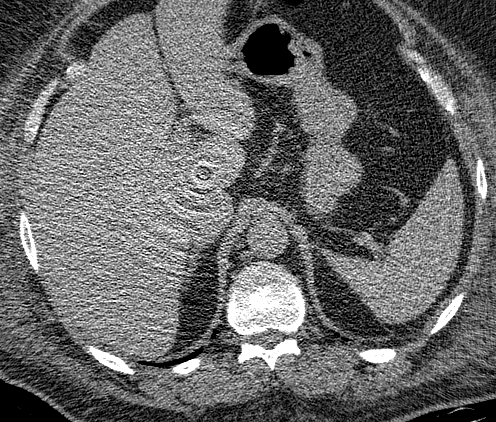
\includegraphics[height=4cm]{images/ring.png}
	\caption{Ring artefact in an abdominal slice\cite{ringArt}}
	\label{ringArtefact}
\end{figure}
\par Ring artefacts are usually obvious and rarely is mistaken for pathology for their perfect circular shape. However they can obscure pathology in affected parts of the scan. Ring artifacts are caused by miscalibrated or defective detector elements, which results in rings as visible in \ref{ringArtefact}. In the sinogram they manifest themselves as lines perpendicular to the projection axis. These artefacts can often be fixed by recalibrating the detector.\cite{ringArt}\cite{CausesAndReductionTechniques}
\par For every detector element a calibration is defined in the form of \(d = ax+b\) where \(b\) is an offset and \(a\) a multiplicative factor.
\par Simulation of miscalibration could be easy: When the ray reaches the detector in the simulation (i.e. the loop over the ray length has finished) not the calculated intensity is added to the result array, but \(d = ax+b\), with random values for \(a\) and \(b\).
\subsubsection{Poisson noise}
\begin{figure}[h!]
	\centering
	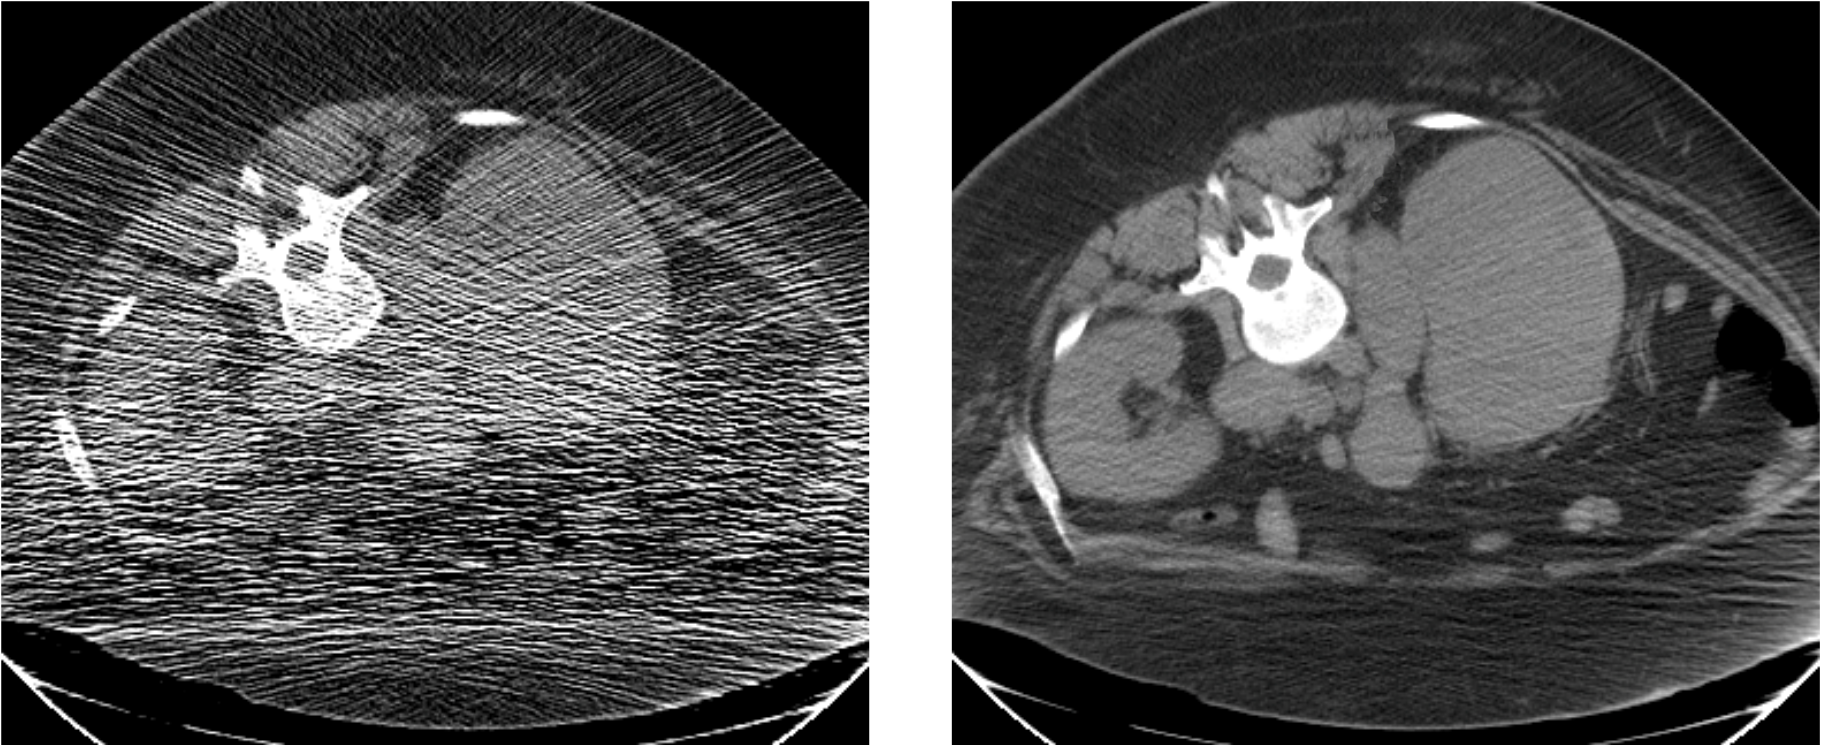
\includegraphics[height=4cm]{images/poisson.png}
	\caption{Abdominal slice of a low dose CT scan on the left showing severe Poisson noise and a high dose scan on the right\cite{CausesAndReductionTechniques}}
	\label{poissonNoise}
\end{figure}
\par \emph{Poisson noise} or \emph{shot noise} is caused by the discrete particle nature of light. Especially at low photon counts i.e. in low dose CT the small fluctuations in the photon count may be enough to result in random thin bright and dark streaks that appear preferentially in the direction of greatest attenuation obscuring soft tissue boundaries as can be seen in \ref{poissonNoise}.\cite{CausesAndReductionTechniques}
\par Simulation of poisson noise should be fairly easy: Instead of randomly modifying the value at the end of the ray as in ring artefacts the relative photon count at the start of the ray can be randomly altered.
\subsubsection{Motion artefacts}
\par Motion artefacts can also happen during a CT scan. They are cause by the patient moving during the scan. Thus some parts of the sinogram are taken with the patient in one position and other parts with the patient in other positions. This causes blurring and double images, as well as long range streaks. Faster scanners reduce motion artefact because the patient has less time to move during the acquisition. An example of motion artefacts can be seen in figure
\begin{figure}[h!]
	\centering
	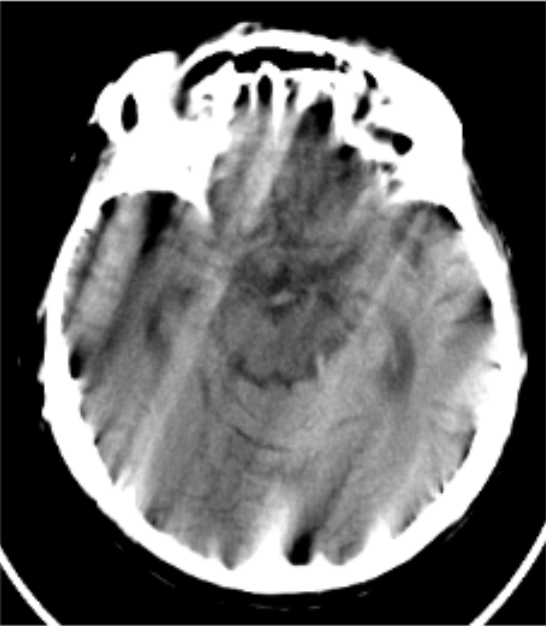
\includegraphics[height=4cm]{images/motion.png}
	\caption{Motion artefact in a brain scan\cite{CausesAndReductionTechniques}}
	\label{motion}
\end{figure}
\par Simulation of motion artefacts can be realized easily: By merging sinogram parts from two or more simulation runs, with the moving object at two slightly different positions.\cite{deMan}

\chapter{Results}
\par This section showcases several images of the simulation. Most of these images took rather long to compute (5-60 minutes) on a 2010 Acer Aspire 3820TG notebook with an Intel Core i5-430M processor and 4GB of RAM. The amount of RAM really shouldn't be a limiting factor, as the simulation usually takes less than 8MB of RAM. Processing power is however crucial as the forward projection completely maxes out all cores of the CPU during the simulation run.
\par Most of these images were created using the same segmented dataset of the Visible Korean Human Project\cite{visibleKorean} with a small metal object placed arbitrarily close to the center of the abdomen.
\par Most of these images are not the original outputs of the simulation, but have their windowing adjusted, so that they look nice and clear. The original images are usually flat and dull, as the windowing just linerly maps all intensities to grey values.
\begin{figure}[h!]
	\centering
	\begin{subfigure}[h]{0.45\textwidth}
		\centering
		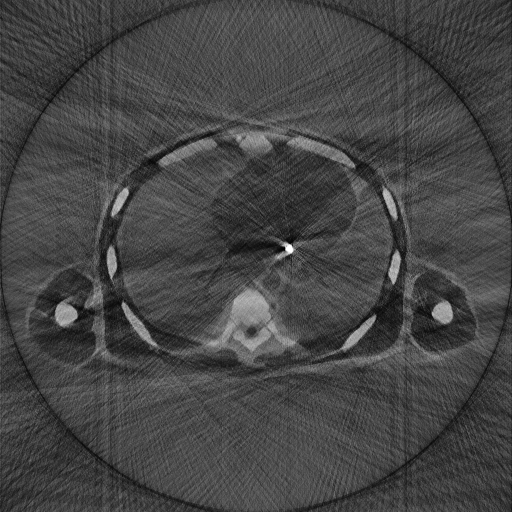
\includegraphics[height=6cm]{images/sim01.png}
		\caption{One simulation run with only slight metal artefacts. Note that even tissue anatomy is visible.}
		\label{sim01}
	\end{subfigure}%
	~
	\begin{subfigure}[h]{0.45\textwidth}
		\centering
		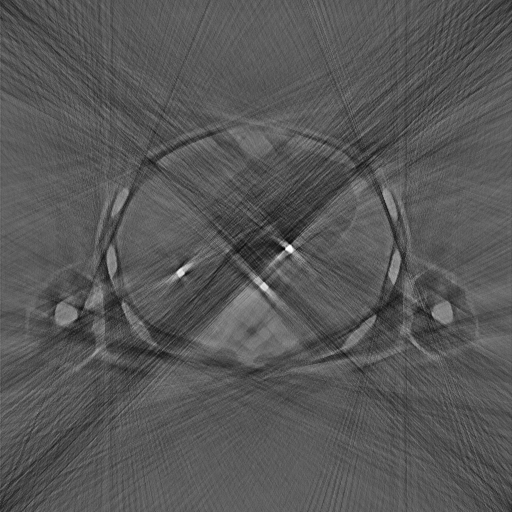
\includegraphics[height=6cm]{images/sim02.png}
		\caption{One simulation run with 3 metal objects placed in the data. Slight metal artefacts are visible as well as string undersampling.}
		\label{sim02}
	\end{subfigure}%
\end{figure}

\begin{figure}[h!]
	\centering	
	\begin{subfigure}[h]{0.45\textwidth}
		\centering
		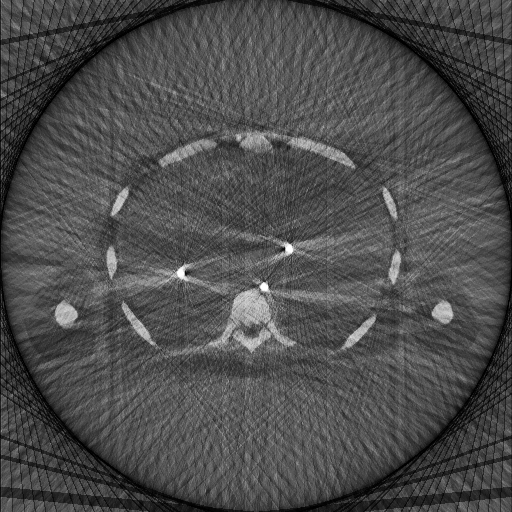
\includegraphics[height=6cm]{images/sim03.png}
		\caption{Another simulation run with 3 metal objects in the dataset. Metal artefacts are more severe in this one.}
		\label{sim03}
	\end{subfigure}%
	~
	\begin{subfigure}[h]{0.45\textwidth}
		\centering
		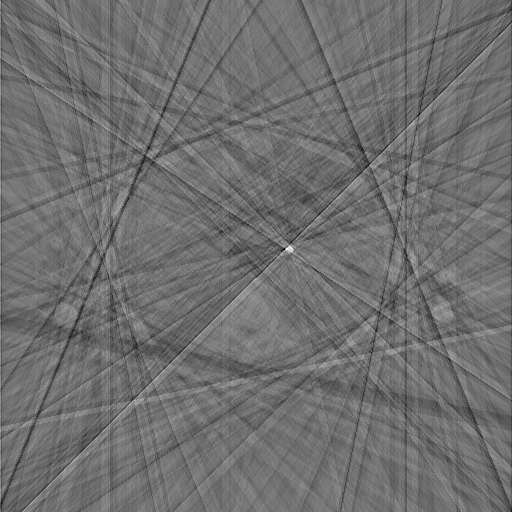
\includegraphics[height=6cm]{images/sim04.png}
		\caption{One 'failed' simulation run. While the metal object is clearly visible, almost no patient anatomy is visible.}
		\label{sim04}
	\end{subfigure}%
\end{figure}

\begin{figure}[h!]
	\centering	
	\begin{subfigure}[h]{0.45\textwidth}
		\centering
		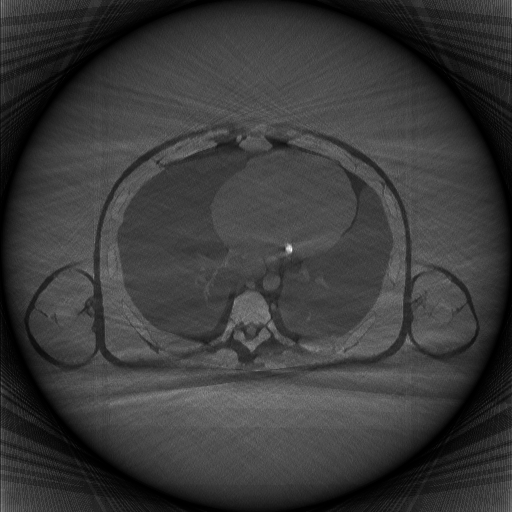
\includegraphics[height=6cm]{images/sim05.png}
		\caption{In this simulation no metal artefacts are visible at all. Patient anatomy is however rendered very clearly and crisp.}
		\label{sim05}
	\end{subfigure}%
	~
	\begin{subfigure}[h]{0.45\textwidth}
		\centering
		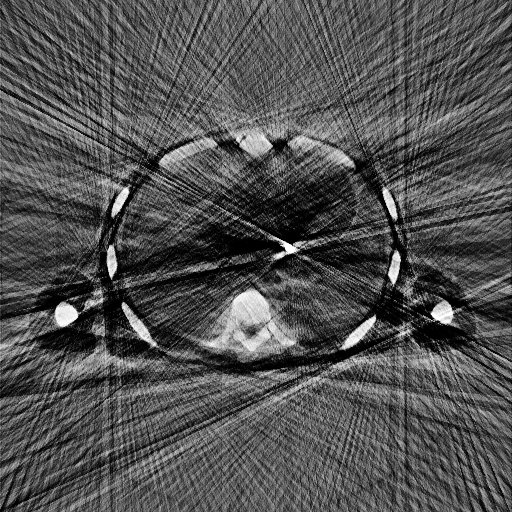
\includegraphics[height=6cm]{images/sim06.png}
		\caption{One of the first simulation runs in which metal artefacts could be seen. Also a lot of undersampling artefacts.}
		\label{sim06}
	\end{subfigure}%
\end{figure}

\begin{figure}[h!]
	\centering		
	\begin{subfigure}[h]{0.45\textwidth}
		\centering
		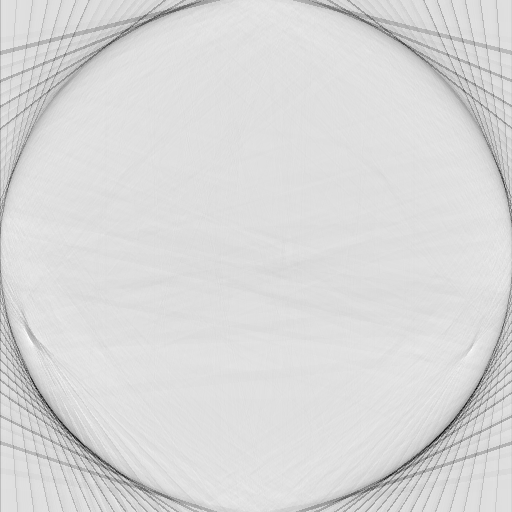
\includegraphics[height=6cm]{images/sim07.png}
		\caption{What can also happen with the simulator: Calculation of the attenuation coefficients was wrong resulting in an almost completely blank image.}
		\label{sim07}
	\end{subfigure}%
	~
	\begin{subfigure}[h]{0.45\textwidth}
		\centering
		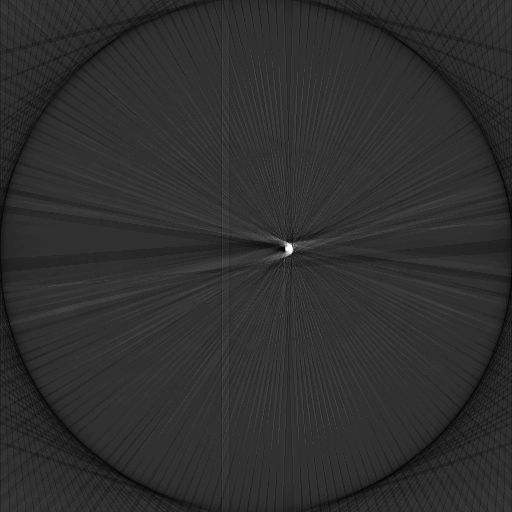
\includegraphics[height=6cm]{images/sim08.png}
		\caption{Another 'failed' run: While the metal object produces nice streaks absolutely no patient anatomy can be seen.}
		\label{sim08}
	\end{subfigure}%
\end{figure}
\chapter{Conclusion}




% ---------------------------------------------------------------------------
%
% Appendix
%
% ---------------------------------------------------------------------------
\part*{Appendix}
\addcontentsline{toc}{part}{Appendix}

\appendix %---------------------------------------
\chapter{Real metal artefacts images for reference}
\label{chapter:RealMetal}

\begin{figure}[h!]
	\centering
	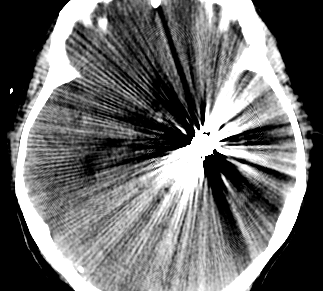
\includegraphics[width=0.5\linewidth]{images/15_FBP.png}
	\caption{Aneurysm clip (with streaks obscuring an acute hemorrhage)\cite{revisionrads}}
\end{figure}
\begin{figure}[h!]
	\centering
	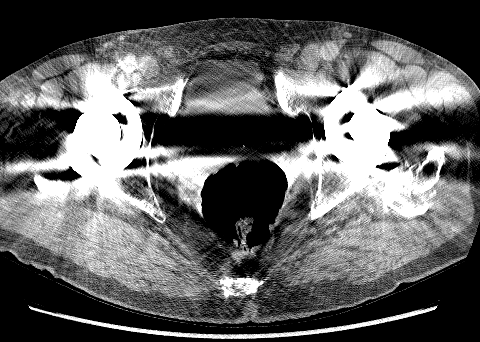
\includegraphics[width=0.5\linewidth]{images/14_FBP.png}
	\caption{Bilateral hip replacements (with streaks obscuring a fluid collection adjacent to the joint)\cite{revisionrads}}
\end{figure}
\begin{figure}[h!]
	\centering
	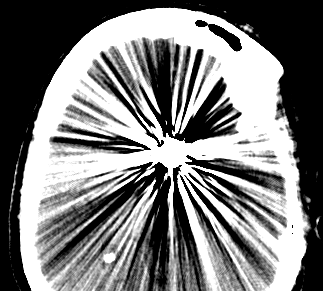
\includegraphics[width=0.5\linewidth]{images/13_FBP.png}
	\caption{Aneurysm clip (with streaks obscuring an acute infarct)\cite{revisionrads}}
\end{figure}
\begin{figure}[h!]
	\centering
	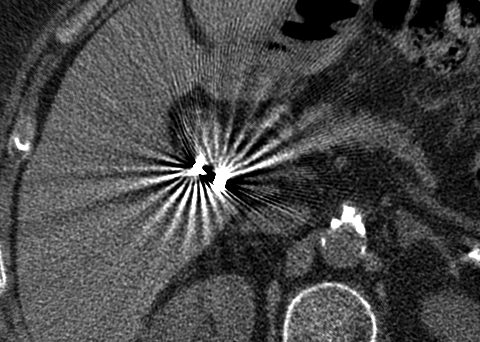
\includegraphics[width=0.5\linewidth]{images/11_FBP.png}
	\caption{Cholecystectomy clips\cite{revisionrads}}
\end{figure}
\begin{figure}[h!]
	\centering
	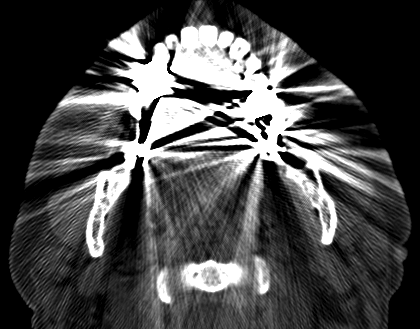
\includegraphics[width=0.5\linewidth]{images/06_FBP.png}
	\caption{Dental fillings\cite{revisionrads}}
\end{figure}
\begin{figure}[h!]
	\centering
	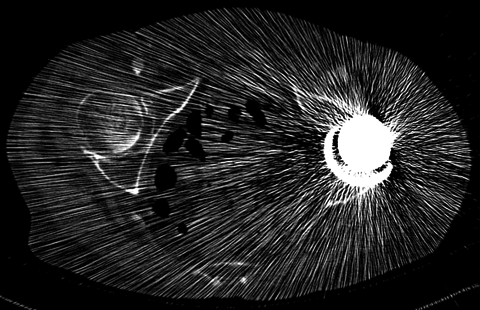
\includegraphics[width=0.5\linewidth]{images/05_FBP.png}
	\caption{Hip replacement\cite{revisionrads}}
\end{figure}
\begin{figure}[h!]
	\centering
	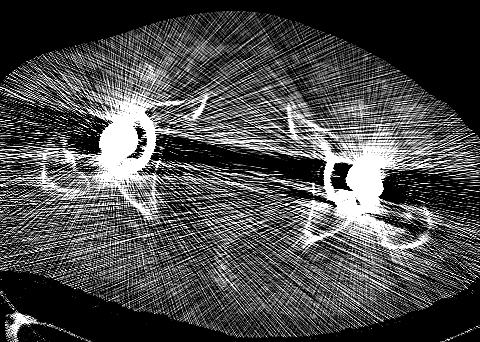
\includegraphics[width=0.5\linewidth]{images/09_FBP.png}
	\caption{Bilateral hip replacements\cite{revisionrads}}
\end{figure}
\begin{figure}[h!]
	\centering
	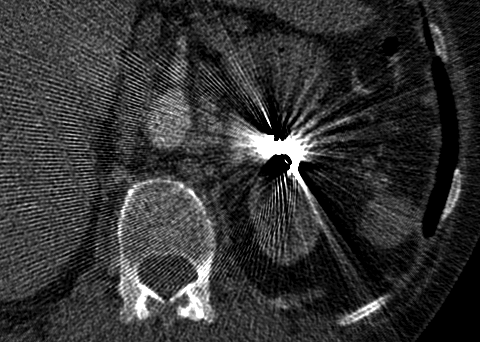
\includegraphics[width=0.5\linewidth]{images/01_FBP.png}
	\caption{Splenectomy clips\cite{revisionrads}}
\end{figure}
\begin{figure}[h!]
	\centering
	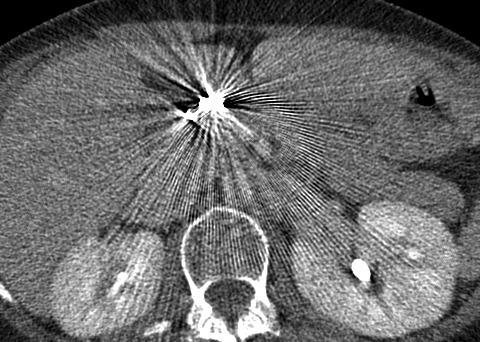
\includegraphics[width=0.5\linewidth]{images/03_FBP.png}
	\caption{Embolization coils\cite{revisionrads}}
\end{figure}
\begin{figure}[h!]
	\centering
	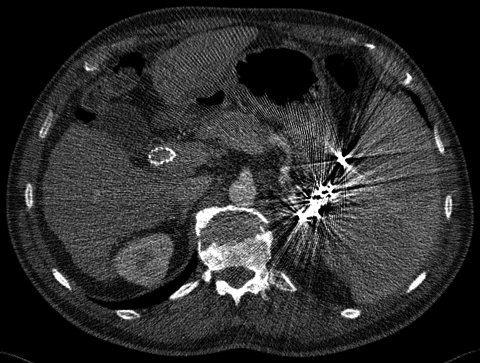
\includegraphics[width=0.5\linewidth]{images/04_FBP.png}
	\caption{Embolization coils\cite{revisionrads}}
\end{figure}